\documentclass[11pt,openany,final]{unsa}
\title{Título}
\author{Nombres y Apellidos}%
\examinerone{Prof. Dr. Nombre Apellido}{Presidente}%
\examinertwo{Prof. Dr. Nombre Apellido}{Secretario}%
\examinerthree{Prof. Dr. Nombre Apellido}{Integrante}%
\examinerfour{Prof. Dr. Nombre Apellido}{Externo}{Universidad del ABC} % of being the case
\date{-}
%\dedicate{ Dedicatoria }
\usepackage{microtype}
\usepackage{caption}
\captionsetup[table]{name=Tabla}

\usepackage{multirow}

\usepackage{listings}
\usepackage{xcolor}




\usepackage{tikz}
\usetikzlibrary{shapes.geometric, arrows.meta, positioning}

\definecolor{codegreen}{rgb}{0,0.6,0}
\definecolor{codegray}{rgb}{0.5,0.5,0.5}
\definecolor{codepurple}{rgb}{0.58,0,0.82}
\definecolor{backcolour}{rgb}{0.95,0.95,0.92}

\lstdefinestyle{mystyle}{
    backgroundcolor=\color{backcolour},   
    commentstyle=\color{codegreen},
    keywordstyle=\color{magenta},
    numberstyle=\tiny\color{codegray},
    stringstyle=\color{codepurple},
    basicstyle=\ttfamily\footnotesize,
    breakatwhitespace=false,         
    breaklines=true,                 
    captionpos=b,                    
    keepspaces=true,                 
    numbers=left,                    
    numbersep=5pt,                  
    showspaces=false,                
    showstringspaces=false,
    showtabs=false,                  
    tabsize=2
    %basicstyle=\linespread{0.8}
}

\lstset{style=mystyle }

\renewcommand{\lstlistingname}{Fragmento de código}
\decimalpoint

\begin{document}%%%%%%%%-------------------------------------------------------
\newcolumntype{L}{>{$}l<{$}}
\newcolumntype{C}{>{$}c<{$}}
\newcolumntype{R}{>{$}r<{$}}
%\makeFirstCover \makeSecondCover %
%\newpage\thispagestyle{empty} \mbox{}%crea una pagina en blanco
\newpage
\thispagestyle{empty}
\begin{doublespacing}       
    \begin{center}
 \hyphenpenalty=10000\Large\uppercase\expandafter{UNIVERSIDAD NACIONAL DE SAN AGUSTÍN DE AREQUIPA}\\
        \hyphenpenalty=10000\large\uppercase\expandafter{FACULTAD DE INGENIERÍA DE PRODUCCIÓN Y SERVICIOS}\\
        \hyphenpenalty=10000\normalsize\uppercase\expandafter{ESCUELA PROFESIONAL DE CIENCIA DE LA COMPUTACIÓN}\\
    \end{center}
\end{doublespacing}
     \null\vskip0.16in
      \begin{center}
         
\includegraphics[scale=0.29]{ESCUDO.jpg}
      \end{center}
          %\begin{center}
         %\includegraphics[scale=0.8]{pg.jpg}\\
         %\small{Maestría en Ciencias de la Tierra}\\

         % \end{center}
    \null\vskip0.16in
    \begin{center}
        \hyphenpenalty=10000\large\expandafter{\textbf{Random Forest para Series
        Temporales de la Actividad Electrodermica de la Piel}}\\
        %\hyphenpenalty=10000\normalsize\uppercase\expandafter{DEL CURSO DE GEOLOGÍA APLICADA A LA
        %INGENIERÍA}\\
        \vskip0.2in
        %\hyphenpenalty=10000\small\uppercase\expandafter{DOCENTE}\\
        %\hyphenpenalty=10000\normalsize\uppercase\expandafter{}

    \end{center}
    \vfill
    \begin{flushright}
\makebox[7cm][l]{Plan de Tesis presentada por:}\\
\makebox[7cm][s]{\textmd{Bejar Merma,Angel Andres } }\\ \vspace{3mm}
\makebox[7cm][s]{Para optar el Título Profesional de:}\\
\makebox[7cm][s]{Licenciado(a) en Ciencia de la Computación}\\\vspace{3mm}
\makebox[7cm][s]{Asesor:}\\
\makebox[7cm][s]{Apellidos, Nombres}\\
\makebox[7cm][l]{}
    %\begin{minipage}[l]{8cm}
       %\small\uppercase\expandafter{Informe presentado por el
      % Bach.\\
      % Efraín Flores Quispe\\
      % para optar el Título Profesional de\\
      % Ingeniéro Geofísico.}
   % \end{minipage}
    \end{flushright}
    \vfill
    \begin{center}
    Arequipa - Perú\\
    2023
    %\today

    \end{center}
    
%\end{doublespacing}
%    \begin{center}
%        \footnotesize Para optar el Grado Académico de \\
%       \uppercase\expandafter{Maestro en Geología} \\
%      en la \\
%        \uppercase\expandafter{Facultad de Geología, Geofísica y Minas,\\
%Universidad Nacional Mayor de San Marcos} \\
%    \end{center}
%    \vskip0.75in
    %\begin{center}
      %  \rm \copyright Copyright por
       % Bach. Joel Ricardo Carrión Rueda\\
        %    \end{center}\newpage
\clearemptydoublepage


%%%%%%%%%%%%%%%%%%%%%%%%%%%%%%%%%%%%%%
\begin{frontmatter}
%\approved{\cuatro}%  {\tres} or {\cuatro}
\dedicatory
\begin{singlespace}
\tableofcontents \listoffigures \listoftables \pagebreak
\end{singlespace}
%\myAcknowledgements{Agradecimientos}%
\myResumen{Resumen}%
%\myAbstrac{Abstract}%
\end{frontmatter}%

\pagestyle{fancyplain}

\chapter{Introducción}
\hrule \bigskip \vspace*{1cm}
%------------------------------------------------------------------------


El estrés es una respuesta natural del cuerpo ante situaciones que percibimos como amenazantes o desafiantes. Esta reacción puede ser de corta duración, conocida como \textbf{estrés agudo}, o prolongarse en el tiempo, dando lugar al \textbf{estrés crónico}. Ambos tipos de estrés tienen efectos significativos en nuestra salud física y mental, aunque sus manifestaciones y consecuencias pueden variar considerablemente.

El estrés agudo se caracteriza por ser una respuesta inmediata y de corta duración ante un estímulo específico. Es el tipo de estrés que sentimos, por ejemplo, antes de un examen importante o durante una situación de emergencia. Aunque puede ser intenso, el estrés agudo suele desaparecer una vez que la situación estresante ha pasado. Este tipo de estrés puede incluso tener efectos positivos, como mejorar el rendimiento y la concentración en situaciones críticas (Smith, 2020).

Por otro lado, el estrés crónico se desarrolla cuando una persona está expuesta a factores estresantes de manera continua o repetitiva. Este tipo de estrés puede tener efectos perjudiciales a largo plazo, contribuyendo al desarrollo de diversas enfermedades, como trastornos cardiovasculares, problemas digestivos y trastornos de ansiedad (Jones \& Brown, 2019). El estrés crónico puede erosionar la salud y el bienestar general, afectando tanto el cuerpo como la mente.

%A lo largo de este artículo, exploraremos en detalle las características y las señales . Finalmente, nos centraremos en la detección del estrés agudo, analizando sus mecanismos, efectos inmediatos y estrategias para su manejo efectivo.

A lo largo de este artículo, exploraremos  las características, causas y consecuencias del estrés agudo y su adquisición mediante la señal EDA. Finalmente, nos centraremos en la detección del estrés agudo utilizando inteligencia artificial, analizando  la señal EDA  y poder  identificar y gestionar eficazmente el estrés %en tiempo real, proporcionando nuevas herramientas para el bienestar y la salud mental.
%%%%%%%
agudo proporcionando nuevas herramientas para el bienestar y la salud mental.




%A pesar de su prevalencia y consecuencias potenciales, el estrés agudo sigue siendo un fenómeno mal entendido. Mientras que el estrés crónico ha recibido una atención significativa en los últimos años, el estrés agudo ha sido ampliamente ignorado, dejando una brecha significativa en nuestra comprensión de sus causas, consecuencias y estrategias de manejo (Harris et al., 2016).



%El estrés agudo es un fenómeno  que afecta a individuos de todas las edades y condiciones. Definido como una respuesta temporal e intensa a una amenaza o peligro percibido (Lupien et al., 2009), el estrés agudo es una respuesta adaptativa normal diseñada para ayudar a los individuos a enfrentar desafíos inmediatos. Sin embargo, cuando el estrés agudo se vuelve excesivo o crónico, puede tener consecuencias devastadoras en la salud física y mental, incluyendo ansiedad, depresión, enfermedad cardiovascular y función cognitiva deteriorada (Kabat-Zinn, 2003; McEwen, 2007).

\section{Justificación}
% ¿ Por qué vale la pena buscar lograr el objetivo planteado?  Se explica los detalles detrás de que la pregunta planteada aún no ha sido respondida, por ejemplo: citar que nadie presentó una solución satisfactoria o que existen soluciones contradictorias.


La detección de estrés agudo es un área de investigación importante y relevante por varias razones:

El estrés en el lugar de trabajo puede afectar significativamente el bienestar del trabajador. Puede llevar a un bajo estado de ánimo y disminución de la atención, lo que puede afectar la calidad de vida del trabajador.

\begin{itemize}
  \item \textbf{Productividad de la empresa:} El estrés no solo afecta al individuo, sino también a la productividad de la empresa. Un trabajador fatigado puede tener un rendimiento reducido, lo que puede afectar la eficiencia y la rentabilidad de la empresa.
  \item Seguridad: El estrés  puede aumentar el riesgo de errores y accidentes. En el caso de los conductores, por ejemplo, la fatiga que deriva en estrés  es una de las principales causas de accidentes de tránsito.
  \item  \textbf{En el campo de la salud:} La detección de estrés agudo es especialmente relevante. Por ejemplo, en pacientes con cáncer, el estrés es un síntoma común que puede afectar en gran medida su vida diaria. Sin embargo, a menudo no se identifica ni se valora adecuadamente, lo que puede resultar en una falta de cuidado y tratamiento adecuados.
  \item \textbf{Investigación en salud:} Por lo tanto, la investigación en la detección de estrés agudo puede tener implicaciones significativas en diversas áreas, desde mejorar la salud y el bienestar de los individuos hasta aumentar la seguridad y la productividad en el lugar de trabajo. Además, puede contribuir a la mejora de las intervenciones y tratamientos en el campo de la salud. Por estas razones, justificar un trabajo de investigación en la detección de fatiga es tanto relevante como necesario.

\end{itemize}


\section{Relevancia y/o Motivación de la Propuesta}




El estrés agudo  se caracteriza como una forma de agotamiento objetivo y subjetivo que surge de la participación prolongada en actividades cognitivas \cite{ishii2014neural}. Tiene implicaciones \cite{grillon2015mental} , \cite{brown2019effects} , \cite{van2017effects} , \cite{dogan2023multi} , \cite{cropanzano2003relationship} sobre las emociones, el comportamiento, el bienestar físico y las interacciones sociales. Los efectos abarcan un espectro de emociones, que incluyen rabia y melancolía , así como una renuencia a participar en entornos sociales.

El estrés agudo es uno de los problemas más comunes que ocurren entre los pacientes \cite{martin2018mental},\cite{marcora2009mental}, en el que un individuo experimenta resistencia a una actividad\cite{meijman2000theory},mal  Humor\cite{hockey1983stress}  letargo \cite{martin2018mental}.
El estrés  se relaciona principalmente con la enfermedad, el envejecimiento
y la depresión.\cite{martin2018mental}.
%La fatiga mental  es un problema que afecta a la sociedad tecnificada hoy en dia .
%\cite{fatiga}

En situaciones de estrés agudo , se observan modificaciones significativas en las señales físicas, como el ritmo cardíaco, la respiración, la sudoración y la dilatación de las pupilas.
En estas situaciones  los dispositivos portátiles se pueden aprovechar para capturar las señales a través  de     sus  sensores, uno de ellos es la pulsera E4 wristband que mide  diversas señales entre ellas EDA ,BVP Figura \ref{fig:relo}.

%La  información que recoje los  dispositivos portátiles son  útiles para ayudar a  detectar fatiga obtener datos valiosos, como los signos fisiológicos de la persona.


%Investigaciones previas han evidenciado que la actividad electrodérmica (EDA), también conocida como respuesta galvánica de la piel (GSR), puede ser indicativa de fatiga mental.EDA registra los cambios en la sudoración al detectar las alteraciones en la conductividad eléctrica de la piel. 

%Aquí se escribe la introducción al problema, yendo de lo más general a lo más específico.

%De preferencia debería iniciarse con la motivación que nos llevó a escoger el problema de la tesis y explicando porque es un problema interesante de resolver.

%En seguida, una vez que se establece claramente cuál es la motivación para resolver el problema, se debe situar el mismo dentro de un contexto. Aquí es donde se debe indicar en que area de la ciencia de la computación está ubicado el problema.

%\textit{
%\textbf{Ejemplo:} Hoy en día debido a la gran cantidad de información generada cotidianamente, y a la caída del costo de los medios de almacenamiento, contamos con grandes bases de datos en muchas empresas (gigabytes o incluso terabytes de datos) ....
%}



La señal electrodérmica de la piel (EDA) mide  los cambios eléctricos en la superficie de la piel, que surgen cuando la piel recibe señales inervantes del cerebro. Para la mayoría de las personas, si experimentan activación emocional, aumento de la carga cognitiva o esfuerzo físico, su cerebro enviara señales a la piel para aumentar el nivel de sudoración ,con ello su posterior registro por medio de los sensores del EDA.
Las unidades de medida de la conductancia son microSiemens.



Las causas del estrés agudo pueden ser variadas, pero algunas de las más comunes incluyen:

\begin{itemize}


  \item \textbf{Exceso de trabajo intelectual:} Las personas que tienen un exceso de empleo de tipo intelectual, donde se les exige comprender, razonar, solucionar problemas, estar concentrados y memorizar de forma casi constante, son propensas a la fatiga mental.

  \item \textbf{Ritmo de vida frenético:} El ritmo de vida acelerado, especialmente en las ciudades, puede llevar al estrés mental.

  \item \textbf{Dificultades para gestionar el tiempo y para desconectar:} La incapacidad para manejar adecuadamente el tiempo y desconectar.


\end{itemize}
%También  se ha estudiado que el estres mental disminuye la conciencia situacional,  aspecto fundamental de la seguridad humana y laboral \cite{kelly2019analysis}.%porque ? %cual son las concecuencia ? 








%¿cual es el ámbito en que esto se desenvuelve? y ¿que necesidad
%existe para motivar una investigación en tu tema?
%Se explica cómo la investigación contribuirá con algo valioso ya sea a nivel científico o social, el impacto que puede tener y por qué es importante que alguien se tome el tiempo para trabajar en esa problemática.


%\section{Pregunta de Investigación}

%Es una pregunta que todavía no fue respondida satisfactoriamente. Debe ser clara, concisa, específica, neutral y enfocada. También deben ser lo suficientemente compleja como para que la pregunta requiera algo más que una respuesta de "sí" o "no", por lo que  usualmente comienza con: ¿Qué … ? ¿Cómo… ?






%\section{Hipótesis}
%La hipótesis es una afirmación de la cual no se sabe si es verdadera o falsa. Es la posible respuesta a la pregunta de investigación. El trabajo de investigación consiste en probar la veracidad de la hipótesis. Es el corazón de la investigación, por lo que una buena hipótesis con evidencia de efectividad debe ser buscada.


\subsection{Definición del Problema}

%Una vez que se indicó la motivación para resolver el problema y fue situado en su respectivo contexto, es necesario dejar claro cuál es el problema que se quiere resolver. Esta sección no debe ser muy larga, ya que se supone que en la sección anterior se hizo toda la introducción necesaria. Idealmente debe ser una sola oración que resuma claramente el problema que se quiere resolver.

%\textit{
%\textbf{Ejemplo:} Se necesita contar con nuevas técnicas que permitan tratar más eficientemente grandes cantidades de información para sistemas computacionales de todo tipo.
%}
%El estres es un que aceja las sosciedad , hoy endai hay dispositivos portatiles que almacena informacion util que ayudan a tener infromacoin valiosa como los signo fisologicos de la prsona  , es por eso que se encesita detectarlo lo mejor posible  posible para obtner patrones que describan su naturaleza 



%A medida que avanza la tecnología  también aumenta la fatiga  , \cite{fatiga} 

%Suele aparecer en situaciones de mucha presión y estrés psicológico, emocional o intelectual. Este cansancio mental  no solo se manifiesta en los pensamientos y la mente, sino que también puede repercutir directamente en el  cuerpo, manifestándose en forma de debilidad física,dolores de cabeza ,dificultar la calidad de sueño\cite{Hockey_2013} ,  u otras complicaciones.

%existen varias limitaciones

Existen varias  limitaciones con respecto a la detección de  estrés agudo.

%Por ejemplo enla validación de  los datos   , los estudios que se  realizaron fueron principalmente en entornos de laboratorio, pero las conclusiones  basadas en laboratorio no necesariamente se aplican a la evaluación  ambulatoria.

Por ejemplo ,en un estudio de laboratorio se  encontró que el 22\% de
los datos de actividad electrodérmica (EDA) recopilados por un dispositivo
portátil eran inutilizables (van Lier et al., 2020), mientras que un estudio
ambulatorio que utilizó el mismo dispositivo estimó el 78\% (van
Lier et al., 2020).

los modelos genericos random forest

%Además  existe poco  estudio donde  se haga un análisis exploratorio de los datos  para visualizar y encontrar  similitudes y diferencias ,dado que  los datos pertenecen a  diferentes  protocolos de estudio como se ha  visto anteriormente.

%es  un estado del organismo que aparece como consecuencia del estrés o de una época puntual de tensión\cite{kelly2019analysis}. 

%Sin embargo,esta poco claro  sus síntomas van más allá y su aparición puede dificultar la calidad del sueño, conllevar problemas musculares y dolores de cabeza



%Actualmente existe trabajos de  investigación que se centran en el  reconocimiento de estrés y a menudo gira en torno al análisis de información fisiológica\cite{dogan2022stress}, \cite{derdiyok2023biosignal}  \cite{parekh2020fatigue}. 


Debido a que el estrés es subjetivo y se expresa de manera diferente de una
persona a otra, los modelos genéricos de predicción del estrés tienen bajo rendimiento. Sólo los específicos
de una persona (dependientes del usuario) producen predicciones confiables, pero no son adaptables y su
implementación en entornos del mundo real es costosa.
Así como  en un entorno de oficina, un modelo  dependiente del usuario requeriría recopilar nuevos datos y entrenar un nuevo modelo para cada empleado. Además, una vez implementados, los modelos se deteriorarían y necesitarían
costosas actualizaciones periódicas porque el estrés es dinámico y depende de factores que no se tienen en cuenta .
%imprevisibles 

%cuál de los enfoques: (dependientes del usuario y los independientes del usuario )sobre la  señal EDA de baja resolución son más precisos para detectar patrones de fatiga.

%Existen mucho modelos de detección de estrés ,usando diversas resoluciones (tasa de frecuencia de muestreo ) Por lo tanto  pero es poco sabido  cual de las dos utiliar   ,este trabajo ara un analisis estadístico de modelos  de  detección de estres de  comparando diversas fuentes de datos 


%Por lo que  el monitorio  podría ayudar a minimizar cualquier consecuencia negativa.

%aca voy a a ser saltar la relevancia del tema porque es importante 















\section{Objetivos}
% ¿Que pretendes obtener o resolver? y en los objetivos específicos
% detallar cada una de las actividades que realizaras, en este punto debes
% ser muy exacto y concreto(recuerda que en base a esto justificaras % si estas obteniendo resultados)

\subsection{Objetivo General}
%El objetivo debe ser directamente verificable al final del trabajo de investigación, un buen objetivo demostrará que la hipótesis que está siendo probada es verdadera o no. Tenga en cuenta que el objetivo no debe ser confundido con el tema de investigación. El objetivo general y los objetivos específicos deben ser formulados de manera que se puedan verificar al final del trabajo, comienzan con verbos en infinitivo, por ejemplo: demostrar, mejorar, analizar.

Diseñar   un sistema para el análisis y la detección de estrés agudo  usando el modelo Random Forest y Perceptrón Multicapa  a partir de la actividad electrodermica de la piel de baja resolución .

Diseñar un modelo  un modelo que mejore la precisión de de los modelos genéricos

\subsection{Objetivos específicos}
%Los objetivos específicos no son etapas de la investigación, son subproductos que serán el resultado del proceso de verificación del objetivo general. Los objetivos específicos deben indicar una contribución.

\textit{
  %\textbf{Ejemplo:}
}

\begin{itemize}

  \item \textit{Preprocesar los datos  }

        %debido a las diferencias en las respuestas fisiológicas de los individuos. }

  \item \textit{Entrenar el modelo utilizando  Random Forest .}

  \item \textit{Identificar   características dominantes  }
        %utilizando la tecnica método One-Leave-Out }
  \item  Comparar los dos  enfoques  utilizando señales EDA de baja resolución.

        %\item Evaluar los resultados del análisis aplicando Cross-Validation 

  \item \textit{Validar la precisión del sistema }

\end{itemize}







%\section{Organización de la tesis}

% Una breve descripción de cada uno de los capítulos que estas
% desarrollando desde el CAP 2 hasta el capitulo antes del apéndice.

\chapter{Marco teórico }

\hrule \bigskip \vspace*{1cm}

%El Marco Teórico es el conjunto de conceptos y bases teóricas necesarias para la comprensión y entendimiento de los diferentes componentes, pasos o etapas planteados en la propuesta del trabajo. Esto permitirá comprender los diferentes conceptos y términos utilizados en todo el trabajo de investigación.
\subsection{SRC y SCL}


La medición de la actividad electrodermica (EDA)  se compone de  dos partes: 

 
\begin{itemize}
    \item \textbf{El nivel de conductancia tónico de la piel(SCL):}Se muestra en la imagen \ref{fig:src}como la señal suave subyacentes que cambia lentamente.
    Se da en ausencia de cualquier evento ambiental discreto particular o estímulos externos. El nivel de conductancia tónica de la piel puede variar lentamente con el tiempo en un individuo dependiendo de su estado psicológico, hidratación, sequedad de la piel.
    \item \textbf{Respuesta  de la Conductancia Cutánea(SRC):}
     Son aumentos bruscos de la conductancia de la piel ,  los picos  en  la Figura \ref{fig:src2}.Se asocian típicamente con eventos a corto plazo y ocurren en presencia de estímulos ambientales discretos: vista, sonido, olfato, procesos cognitivos que preceden a un evento, como anticipación, toma de decisiones, etc. 
\end{itemize}

\begin{figure}[h]
    \centering
    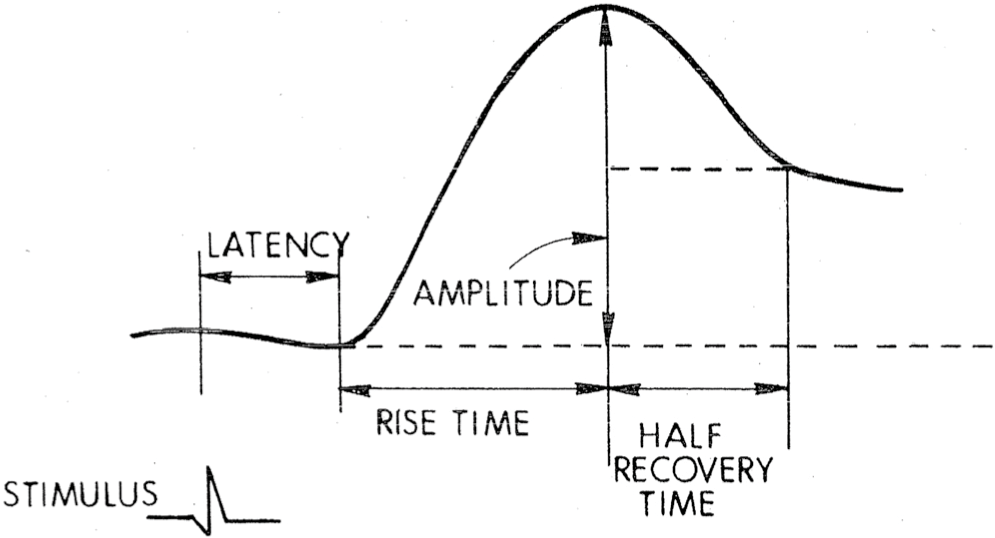
\includegraphics[width=10cm]{Graficos/senal.png}
    \caption{ Visualización de los componentes de un SRC ante un evento .Dawson et al.[Dawson et al,2017] }
    \label{fig:src2}
\end{figure}

\begin{figure}[h]
    \centering
    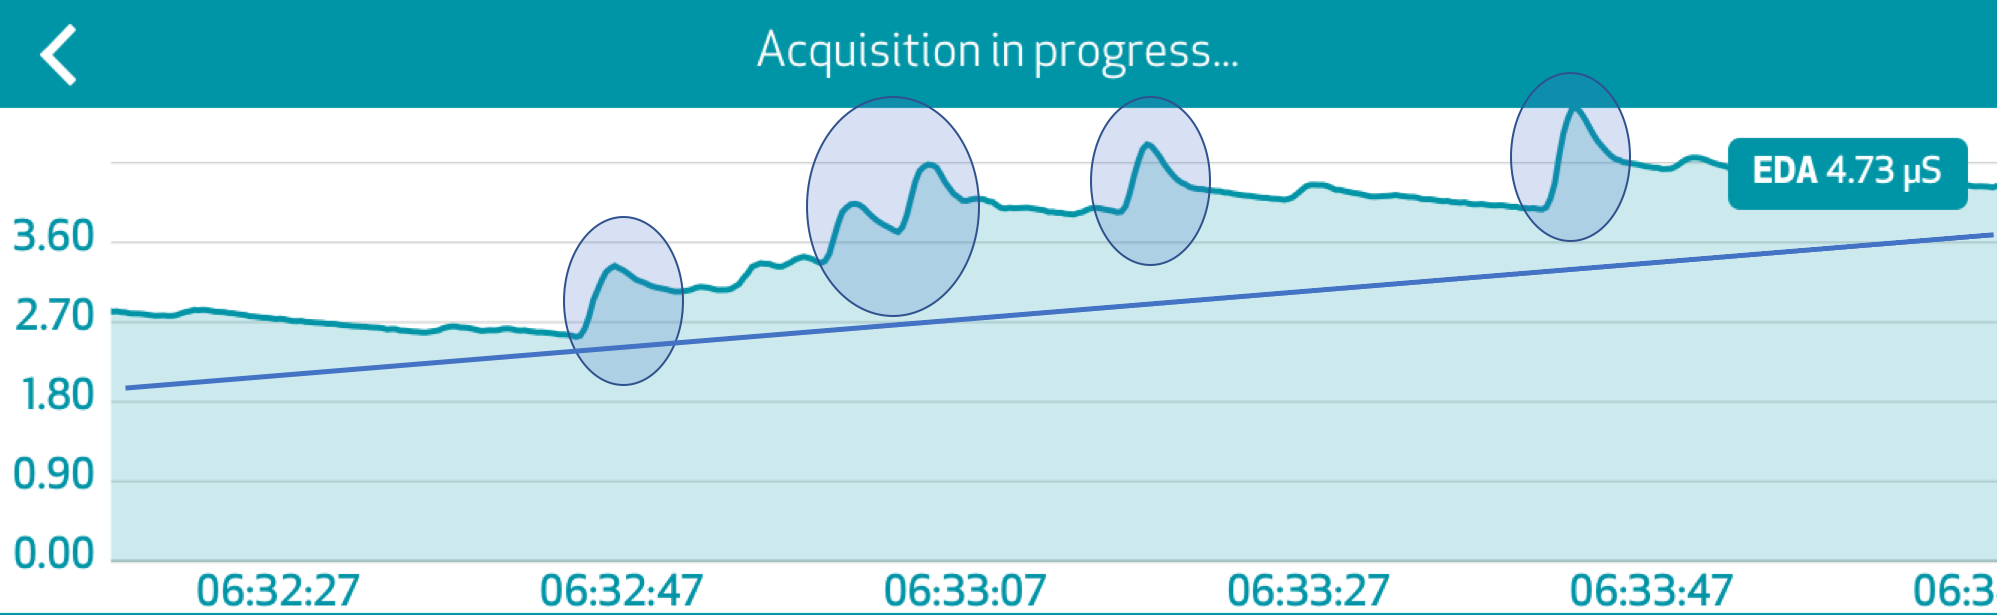
\includegraphics[width=15cm]{Graficos/new_EDA_figure.png}
    \caption{ Señal EDA capturado de la Aplicación Empatica Realtime}
    \label{fig:src}
\end{figure}

\begin{figure}[h]
    \centering
    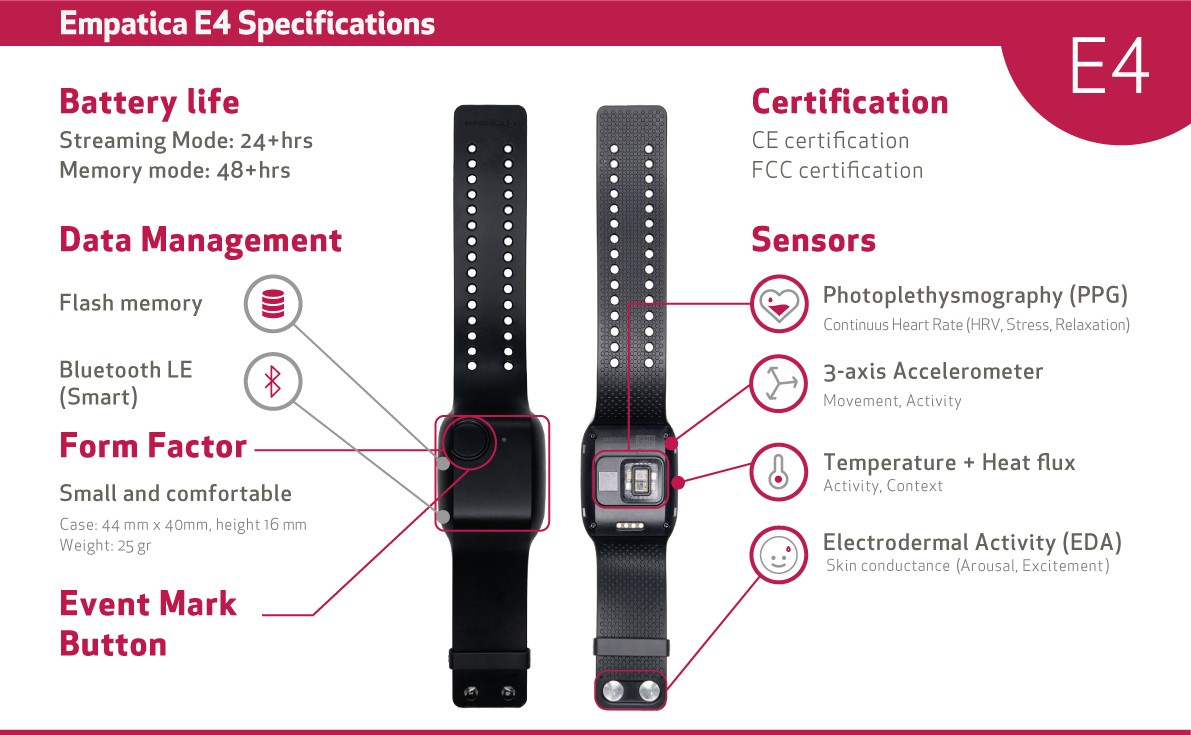
\includegraphics[width=15cm]{Graficos/e4specs.jpg}
    \caption{ Especificaciones técnicas del E4-wristband}
    \label{fig:relo}
\end{figure}

    
    
    
\chapter{Estado del Arte }

\hrule \bigskip \vspace*{1cm}

%La revisión bibliográfica o el estado del Arte son trabajos, publicaciones o propuestas similares realizadas por otros autores que tratan de resolver el mismo problema planteado en el trabajo de tesis pero con diferentes herramientas, métodos o experimentos. No es necesario una descripción al detalle de todos los trabajos de investigación similares encontrados, el estado del arte debe ser preciso y conciso en cuanto al modo de resolver cierto problema, las herramientas utilizadas, los resultados obtenidos y ventajas o desventajas identificadas. Toda esta información ayudará a comprender y contextualizar el área de investigación seleccionada.

Existen diversos trabajos en donde se proponen detectar  estrés agudo,estos trabajos utilizan diferentes métodos los cuales se pueden implementar a través de modelos matemáticos ,modelos Deep learning ,modelos de Maching Learning.

\subsection{ Maching Learning
} En  \cite{bai2021towards} hicieron un análisis donde usaron  el modelo  Random Forest basados en  efectos mixtos  en donde 
extrajeron características de cada modalidad  para aprovechar la información demográfica y  mejorar el rendimiento. Los resultados que obtuvieron con los experimentos del   conjunto de datos que recopilaron fueron prometedores. Sugirieron que el ECG(Electrocardiograma) es la señal mas importante en la detección de fatiga.









\subsection {Por reglas definidas }

\cite{devi2010fuzzy} sugirió la  técnica FIS (Fuzzy Inference Systems ) para la detección de la fatiga, en la que los estados de la boca y los ojos se utilizaron como entrada , para predecir  el estado del conductor ,ya sea  peligroso, fatigado o normal. Dividieron los estados oculares en categorías: parpadeo, cerrado o somnoliento. Mientras que los estados de la boca se clasificaron como normales o bostezos. Otra investigación\cite{sikander2018driver} ha tenido en cuenta las características mencionadas anteriormente y ha desarrollado una técnica para detectar la fatiga utilizando un FIS de dos capas.

En la detección  de fatiga mediante aprendizaje automático,existe el trabajo de \cite{fan2007yawning} que utilizo el bostezo como parámetro ,sugirió un método para rastrear el movimiento de la cara con la ayuda de una cámara. En la técnica   (Gravity-Centre) propuesta por el autor  para detectar las comisuras de la boca utilizando  proyección de grises , extrajo las características de la boca mediante el uso de ondículas de Gabor que produjeron información sobre órganos como los ojos, la nariz, la boca y los labios. utilizaron  ondícula de Gabor de representación bidimensional para analizar y procesar la textura de la imagen. Luego, utilizó el análisis discriminante lineal (LDA) para clasificar los vectores de características con el fin de detectar la guiñada.

La técnica que propusieron  fue evaluada sobre 400 imágenes y 20 videos que constaban de 4512 rostros. Las características de Gabor fueron capaces de detectar bostezos con una precisión del 96\%, mientras que las características geométricas fueron capaces de detectar bostezos con una precisión del 69,5\%.Finalmente concluyeron que los coeficientes de gabor son más eficientes que las características geométrica.





\subsection{Detección de fatiga mediante Gradient Boosting Decision Tree (GBDT)}


\cite{hu2018automated} Trató de detectar las características de las señales de EEG, mediante el cálculo de conjuntos de características que incluían las entropías, como una muestra, espectral, difusa y aproximada. Los autores utilizaron la técnica   Gradient Boosting Decision Tree (GBDT)  basado en una estrategia codiciosa ,llamada aumento de gradiente, que tenían como entrada las características de EEG . Para evaluarlo, utilizaron tres clasificadores ampliamente conocidos, a saber, K-vecinos más cercanos (KNN), SVM, ANN para la comparación.

Además, los autores realizaron experimentos en 22 seres humanos. Inicialmente, se les pidió que practicaran la conducción durante varios minutos para familiarizarse con el sistema. La duración de los experimentos realizados fue de unos 40-120 minutos. Los resultados de estos experimentos demostraron que fue posible lograr una precisión de hasta el 95\% para detectar la fatiga mediante EEG.



\subsection{Detección de fatiga mediante aprendizaje profundo}
Por otro lado en el aprendizaje profundo
\cite{du2017detecting} propuso un enfoque multimodal mediante la combinación de EEG y electrooculograma (EOG) para detectar la fatiga. Las señales fisiológicas se utilizaron ampliamente para detectar el estado de los seres humanos.
Por medio de  la amplitud dedujeron  que las  señales  EOG son más efectivas contra el ruido.   %La amplitud de las señales EOG en comparación con las señales EEG es mayor, por lo que las señales EOG son más efectivas contra el ruido.
Además , los autores introdujeron un modelo  multimodal de autoencoder  para la detección de fatiga. El modelo que presentaron  utilizo señales de EEG y EOG. El experimento se realizó en personas a las que se les pidió que condujeran durante al menos 2 horas ,se capturaron las señales de EOG y EEG utilizando un sistema NeuroScan y se utilizó SVM junto con la función de base radial (RBF) como modelo de regresión.


%Para medir la eficiencia de la técnica de fusión, los autores entrenaron dos modelos unimodales solo con señales de EEG y EOG. El resultado de esto se comparó con otro modelo entrenado con estrategias de fusión. El resultado del experimento sugirió que el modelo de fusión de características funciona mejor que el modelo entrenado en características individuales. 

Finalmente la precisión que obtuvieron  del modelo    auto-encoder multimodal   fue de 85\%.


\cite{computation7010013}  Desarrollo técnicas de última generación para detectar etapas de somnolencia en EEG (la mejor medición fisiológica). Se utilizo un bloque de Transformada de Coseno Discreto (DCT) para realizar la transformación en la frecuencia muestral de EEG. Utilizaron un autoencoder para descubrir patrones de datos no supervisados junto con la reducción de dimensionalidad.

Los resultados que obtuvieron    fueron 100\% precisos cuando se probaron en 62 individuos, dominando todas las metodologías anteriores y prometiendo una utilidad en las futuras generaciones de dispositivos médicos.

%Se utiliza un bloque de transformada discreta de coseno (DCT) para realizar la transformación en el dominio de la frecuencia de las muestras de EEG. A continuación, los resultados se redimensionan mediante una reasignación bicúbica constituida por 256 muestras. El resultado transformado se convierte en una matriz unidimensional que consta de 256 muestras de frecuencia. Las entradas para las capas del autocodificador fueron señales de frecuencia optimizadas de EEG generadas a partir de DCT. Un codificador automático se utiliza para descubrir patrones de datos no supervisados junto con la reducción de la dimensionalidad. Con el fin de aumentar la eficiencia del sistema, se considera un enfoque codicioso por capas (Fig. 3).



\begin{center}
    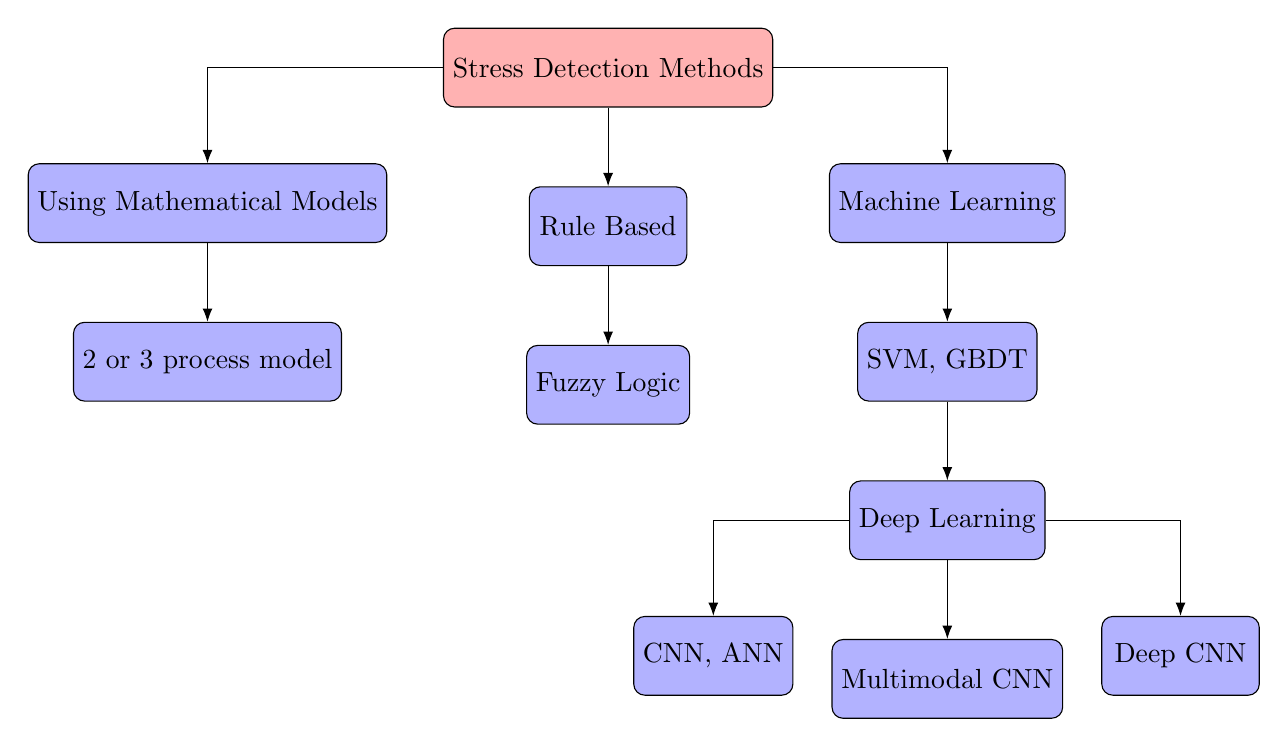
\begin{tikzpicture}[node distance=1cm, auto]
    
    % Define style for boxes
    \tikzstyle{main} = [rectangle, rounded corners, minimum width=3cm, minimum height=1cm,text centered, draw=black, fill=red!30]
    \tikzstyle{sub} = [rectangle, rounded corners, minimum width=2cm, minimum height=1cm, text centered, draw=black, fill=blue!30]
    
    % Nodes
    \node (fatigue) [main] {Stress Detection Methods};
    \node (mathmodels)[sub, below left=of fatigue] {Using Mathematical Models};
    \node (rulebased) [sub, below=of fatigue] {Rule Based};
    \node (machinelearn) [sub, below right=of fatigue] {Machine Learning};
    
    \node (fuzzylogic)[sub, below=of rulebased]{Fuzzy Logic};
    %\node (deeplearn) [sub, below right=of fatigue]{Deep Learning};
    
    \node (processmodel) [sub, below=of mathmodels] {2 or 3 process model};
    %\node (fuzzylogic) [sub, below=of processmodel] {Fuzzy Logic};
    \node (svmgbdt) [sub, below=of machinelearn] {SVM, GBDT};
    
    
    \node (deeplearn) [sub, below=of svmgbdt] {Deep Learning};
    
    
    \node (cnnann) [sub, below left=of deeplearn] {CNN, ANN};
    \node (multimodalcnn) [sub, below=of deeplearn] {Multimodal CNN};
    \node (deepcnn) [sub, below right=of deeplearn] {Deep CNN};
    
    % Lines
    \draw[-Latex] (fatigue) -| (mathmodels);
    \draw[-Latex] (fatigue) -- (rulebased);
    \draw[-Latex] (fatigue) -| (machinelearn);
    %\draw[-Latex] (fatigue) -| (deeplearn);
    
    \draw[-Latex] (mathmodels) -- (processmodel);
    \draw[-Latex] (rulebased)--(fuzzylogic);
    %\draw[-Latex] (processmodel) -- (fuzzylogic);
    \draw[-Latex] (machinelearn) -- (svmgbdt);
    \draw[-Latex] (svmgbdt) -- (deeplearn);
    
    \draw[-Latex] (deeplearn) -| (cnnann);
    \draw[-Latex] (deeplearn) -- (multimodalcnn);
    \draw[-Latex] (deeplearn) -| (deepcnn);
    
    \end{tikzpicture}
    
    
    
    \end{center}
    
    
    
    \begin{center}
    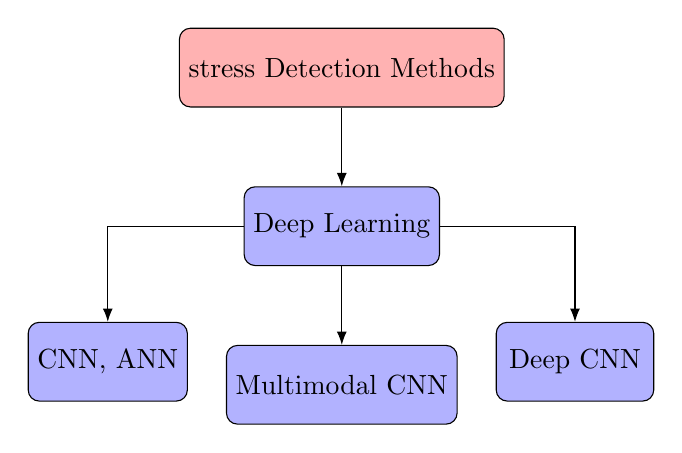
\begin{tikzpicture}[node distance=1cm, auto]
    
    % Define style for boxes
    \tikzstyle{main} = [rectangle, rounded corners, minimum width=3cm, minimum height=1cm,text centered, draw=black, fill=red!30]
    \tikzstyle{sub} = [rectangle, rounded corners, minimum width=2cm, minimum height=1cm, text centered, draw=black, fill=blue!30]
    
    % Nodes
    \node (fatigue) [main] {stress Detection Methods};
    \node (deeplearn)[sub, below =of fatigue] {Deep Learning};
    
    \node (cnnann)[sub, below left =of deeplearn] {CNN, ANN};
    \node (multimodalcnn)[sub, below =of deeplearn] {Multimodal CNN};
    \node (deepcnn)[sub, below right =of deeplearn] {Deep CNN};
    
    
    
    
    % Lines
    \draw[-Latex] (fatigue) -- (deeplearn);
    
    %\draw[-Latex] (fatigue) -| (deeplearn);
    
    
    \draw[-Latex] (deeplearn) -| (cnnann);
    \draw[-Latex] (deeplearn) -- (multimodalcnn);
    \draw[-Latex] (deeplearn) -| (deepcnn);
    
    \end{tikzpicture}
    
    
    
    \end{center}
    
    



\begin{table}[h!]
    \centering
    \caption{Resumen de todas las metodologías para la detección de estrés .}
    \label{tab:metodologias}
    \begin{scriptsize} % Reduce the font size
    \begin{tabular}{|l|l|l|l|}
    \hline
    \textbf{Tipos de Características} & \textbf{Modelo de Extracción de Datos} & \textbf{Precisión} & \textbf{Datos} \\ \hline
    
    Detección de bostezos            & Coeficientes de Gabor                                 & 95\%               & 400 images \cite{fan2007yawning}              \\ \hline
    
    Estado del ojo                    & AdaBoost                             & 90.18\%            &    2100 images \cite{wang2010novel}             \\ \hline
    
    Señales EEG                       & Árbol de Decisión Potenciado         & 95\%               &   Serie Temporal\cite{hu2018automated}            \\ \hline
    
    Comportamiento facial             & SVM                                  & 94.8\%             &     Imagenes iBUG 300-W\cite{carass}       \\ \hline
    
    registros EEG            & Neural Network                                  & 83.6\%             &  del MIT-BIH\cite{national2011fars}            \\ \hline
    
    EEG (Tiempo Real)              &Linear Regression                                 & 90\%             &       Tiempo Real         \\ \hline
    
    
    Skin conductance            &SVM                                 & 92.95\%             &  Imágenes  \cite{bundele2009svm}
               \\ \hline
    
    EDA             &Estadístico basado en  la excitación                                   & 79.17\%           &  Series de Tiempo               \\ \hline
    
    EDA y audio             &SVM y ANN                                   & 88.8\%           &   Wesad\cite{Schmidt2018IntroducingWA}               \\ \hline
    
    EEG            &Autoencoder  y DCT                                 & 100\%           &   \cite{computation7010013}               \\ \hline
    
    multimodal            &modelo random forest-based mixed-effects,                                 & 0.75            &   \cite{10.1145/3460421.3480429}               \\ \hline
    
    %EDA+BVP+ST            &NN                           & 94.16\%            &   \cite{10.1007/978-3-031-08530-%7_77}               \\ \hline
    
    EDA+HR          &AcRoNN                           & 86.87\%            &   \cite{alam2021activity}               \\ \hline
    
    ECG, EDA,EMG  ,EEG          &LSTM, RF                           & 84.1\%            &   \cite{Jaiswal2022AssessingFW}               \\ \hline
    
    EDA            & ADA-bosst                        & 97.03\%            &   \cite{9995093}               \\ \hline
    
    ECG           & CNN                   &  98.57\%            &   WESAD\cite{YING2023763}               \\ \hline
    
    Multimodal           & SELF-CARE                  &  94.12\%            &   WESAD\cite{rashid2023stress}               \\ \hline
    
    
    \end{tabular}
    \end{scriptsize} % End of font size reduction
    \end{table}
    
    
    
\chapter{Propuesta}
\hrule \bigskip \vspace*{1cm}
%------------------------------------------------------------------------

% La propuesta es la descripción detallada de las secuencias de etapas, pasos o instrucciones a seguir para lograr demostrar una hipótesis o alcanzar un objetivo planteado. Se debe incluir diagramas que permitan visualizar todo el proceso propuesto para mejorar la comprensión de la idea planteada.
% La propuesta debe responde las siguientes preguntas:
% ¿Cómo se puede lograr el objetivo?
% ¿Cuál es la secuencia de pasos a seguir para lograr alcanzar el objetivo general planteado?
% 	En caso de haber planteado una hipótesis, la propuesta debe demostrar la secuencia de pasos o actividades a ser realizados para verificar si la hipótesis es verdadera o falsa.



\begin{figure}[h]
    \centering
    \includegraphics[width=15cm]{Graficos/Azul y Blanco Diagrama de Flechas Presentación2.png}
    %\caption{Caption}
    \label{fig:enter-label}
\end{figure}


\begin{itemize}
    \item \textbf{Preprocesamiento:}
En esta etapa, se preparan los datos antes de alimentarlos al modelo de aprendizaje automático. Esto puede incluir:
\textbf{Limpieza de datos:}
Utilizando \cite{DERDIYOK2024109896} se eliminar valores atípicos, completar datos faltantes con  interpolación lineal ,eliminar datos inconsistentes .
\textbf{Filtro:} Se aplica un filtro  Butterworth low-pass filter de 5HZ   .
\textbf{Normalización:} Escalar los datos para que tengan una escala similar Min-max scaling.



    \item \textbf{Detección de características:}
Aquí se extraen características relevantes de los datos.
Se usa  técnicas como:
CVxEDA: parar separar los  componente de la señal EDA en  componente tónico y fasico.
También se  extraen las características estadísticas 


    \item \textbf{Entrenamiento y Clasificación:}
\textbf{Se divide los datos } en entrenamiento y prueba  .
En esta etapa,se utiliza dos algoritmos ,Random Forest y  Redes neuronales, también se encuentra los óptimos Hyperparametros con GridSearch. El modelo ajusta sus parámetros para minimizar el error en las predicciones.

    \item \textbf{Análisis:}
Implica analizar la variabilidad de las propiedades estadísticas la diferencias y similitudes de los dataset .

    \item \textbf{Validación:}
Se evalúa el rendimiento del modelo utilizando datos de prueba.

Se utiliza la Validación cruzada para evaluar el rendimiento de manera robusta.
Se utiliza Métricas de evaluación  como precisión, recall,y se compara con otros estudios similares .



\end{itemize}


Por tanto  se propone  el diseño de  un sistema  para la detección de estrés    a partir de datos fisiológicos EDA de baja resolución.
%y realizar el análisis comparativo  de los datos en entornos de laboratorio .  


\subsection*{ DatabaseWork3d}

El conjunto de datos contiene muestras de situaciones de trabajo fatigantes y libres de estrés,proporciona una representación  de varios niveles de estrés. El conjunto de datos se acompaña de metadatos y anotaciones extensas, que facilitan el análisis e interpretación en profundidad. 

Contiene  datos de actividad electrodérmica (EDA), presión volumétrica sanguínea (BVP), temperatura de la piel y acelerómetro (ACC). EDA se muestrea a 4 Hz y abarca aspectos de conductividad de la piel, fásicos y tónicos, que se distinguen por un umbral de aproximadamente 0,05 ms. La temperatura de la piel se registra constantemente a 4 Hz en grados Celsius. 
Los datos de presión arterial se derivan de la señal del pulso de volumen sanguíneo (BVP) de 64 Hz. Los datos del acelerómetro se recopilan a 64 Hz para medir la fuerza gravitacional (g) en las tres dimensiones espaciales (x, y y z). 

Estas señales se capturan utilizando sensores de pulsera Empatica E4 y se aplica una técnica de reducción de resolución(downsampling) para estandarizar las frecuencias, equilibrando un examen fisiológico exhaustivo. 
y seguimiento continuo de la actividad. La opción de reducción de resolución, que reduce todas las entradas a 4 Hz, garantiza un conjunto de datos consistente y efectivamente fusionado.


\begin{figure}[h]
    \centering
    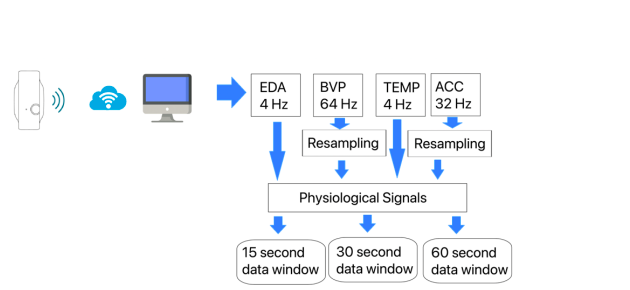
\includegraphics[width=7cm]{Graficos/captura3.png}
    \caption{dataset work3d}
    \label{fig:enter-label}
\end{figure}


\subsection*{Database 2}
Desde un primer momento se utlizara  los conjuntos de datos WESAD, Work3d para probar las hipótesis. Los  conjuntos de datos se utilizan para comparar estadísticamente la precisión de la detección de estrés de los modelos independientes y dependientes del usuario .

Conjunto de datos WESAD: El conjunto de datos publicado consiste en datos fisiológicos recopilados de 15 participantes bajo dos protocolos de estudio diferentes que incluían una combinación de condiciones de diversión/estrés/relajación.




Los archivos del dataset  en su forma natural contienen  información derivada  que en  este estudio se ignoraran : HR.csv, IBI.csv, tags.csv. El archivo info.txt contiene algunos detalles sobre el contenido de la carpeta. Los datos sin procesar del dispositivo E4 están contenidos en los siguientes archivos (en cada archivo, la primera línea se refiere a la marca de tiempo global del canal del sensor al inicio, la segunda línea se refiere a la frecuencia de muestreo del canal del sensor).

\begin{itemize}
    \item ACC.csv: muestreado a 32 Hz. Las 3 columnas de datos se refieren a los 3 canales del acelerómetro. Los datos se proporcionan en unidades de 1/64 g.
    \item BVP.csv: muestreado a 64 Hz. Datos de fotopletismógrafo (PPG).
    \item EDA.csv: muestreado a 4 Hz. Los datos se proporcionan en $\mu$ S.
    \item TEMP.csv: muestreado a 4 Hz. Los datos se proporcionan en grados centigrados .
\end{itemize}

En el experimento ,el dispositivo E4 fue usado en el 
muñeca no dominante de los participantes. La tasa de muestreo de los diferentes sensores fue diferente.
Tambien se registro modalidades de pulso de volumen sanguíneo (BVP) fisiológico de alta resolución, electrocardiograma (ECG), actividad electrodérmica (EDA), electromiograma (EMG), respiración (RESP), temperatura de la piel (TEMP) y movimiento (ACC) con el dispositivo  llamado RespiBAN. Al mismo tiempo, también los participantes usaron la  pulsera Empatica E4 para capturar datos EDA de baja frecuencia de muestreo . 





\subsection{Preprocesamiento}
\begin{figure}
    \centering
    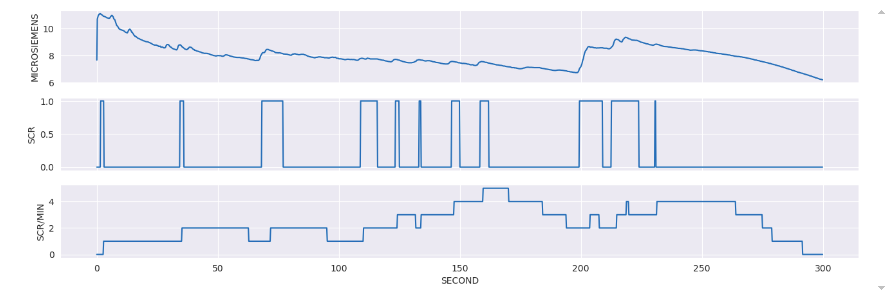
\includegraphics[width=10cm]{Graficos/captura2.png}
    \caption{Caracteristicas}
    \label{fig:enter-label}
\end{figure}


\subsection*{Extracción estadística de características EDA}

La señal EDA se filtró a través de un filtro  Butterworth low-pass filter de cuarto orden de 5 Hz. Lo que significa que sólo la señal EDA de alta resolución de los datos de WESAD-Chest se preprocesa a través de  el filtro  antes de extraer las características . A continuación se extrajeron las características de Eda QUE comprender la respuesta de conducción cutánea (SCR ),nivel de conducción cutánea ,los picos de scr, inicios scr ,y la amplitud scr. junto con  las características estadísticas .El tamaño de ventana y el desplazamiento de ventana fueron de 60 segundos y 30 segundos respectivamente lo que significa que  el modelo busca patrones de estrés después de cada 30 segundos mediante la observación de características estadísticas extraídas  en el paso anterior  en el intervalo de 60 segundos.


\subsection{Entrenamiento}

Utilizando las características estadísticas, se entreno  un modelos de aprendizaje automatico para detectar  estrés : RAndom Forest (RF),y multi- Perceptrón de capa (MLP), utilizando Grid Search .La estandarización de la característica  se aplica para la entrada de MLP, ya que el  modelo funcionan mejor  con datos estandarizados.
Se realizo la estrategia Leave-One-Group-Out (LOGO) para el modelo de detección de estrés independiente del usuario.
 Los datos de entrenamiento y prueba para el entrenamiento dependiente del usuario se dividen mediante   stratified train-test split strategy  (entrenamiento y prueba) cuyo tamaño de prueba es igual al 28,6 \%



\begin{table}[h!]
  \centering
  \caption{Configuraciones de Grid Search de cinco modelos de Aprendizaje Automático utilizados al entrenar modelos de detección de estrés.}
  \label{tab:GridSearchConfiguration}
  \begin{tabular}{|c|c|c|}
    \hline
    \textbf{Modelo} & \textbf{Parámetros GridCV} & \textbf{Valores} \\
  
    \hline
    RF & n\_estimadores & 500, 1000 \\
    & Mínimo de muestras para dividir & 2, 4 \\
    & Mínimo de muestras por hoja & 1, 4 \\
    & Peso de clase & Ninguno, balance \\
    \hline
    MLP & Tamaños de capas ocultas & 64, 128, 256, 512 \\
    \hline
  
  \end{tabular}
\end{table}




\subsection{Análisis}

Lo que se espera es que el modelo dependiente del usuario detecte estadísticamente patrones con mayor precisión que un modelo  independiente del usuario,independientemente  de la elección del modelo de aprendizaje automático.
Se entrenaron 2 modelos independientes y 2 modelos dependientes  configurando LOGO junto con  GridsearH,la métrica  BA son calculados para cada individuo en cada Dataset para crear puntuaciones de evaluación de los modelos independientes y dependientes del usuario respectivamente.
Los datos contienen 2x2(número de modelos)x35 observaciones para ambas salidas ,modelos dependientes y independientes del usuario.
Cada uno consta de resultados independientes  de 2 modelos de aprendizaje automático x35 datos de participantes en 2 conjuntos de datos .

En el  experimentos, nos  enfocamos  en cubrir el análisis usando  estadística inferencial,sobre la población utilizando  un número de  muestras representativas. Se utiliza , la prueba de hipótesis  para estimar el desempeño estadístico de los modelos de detección de estrés  independientes y dependientes del usuario.

 A partir de este punto, las hipótesis nula y alternativa de la prueba unilateral de suma de rangos se 
establecen de la siguiente manera:
\begin{itemize}
    \item  H0 : M1 = M2 (El modelo dependiente del usuario no mejora en distinguir patrones estresantes y no estresantes).
    \item Ha : M1 > M2 (El modelo dependiente del usuario logra distinguir patrones de estrés/no estrés
 de forma  más precisa que uno independiente del usuario).
\end{itemize}

donde , M1 y M2 indican la mediana de las puntuaciones de precisión de la predicción 
de estrés/sin estrés de los modelos dependientes e independientes del usuario.







%\chapter{Cronograma de Actividades}
\hrule \bigskip \vspace*{1cm}
%------------------------------------------------------------------------

%Diagrama de gantt
\chapter{Experimentos y Resultados}
\hrule \bigskip \vspace*{1cm}
%------------------------------------------------------------------------

En este trabajo, se considero  los datos de uso en el pecho como WESAD-Chest y los datos de uso en la muñeca como WESAD-Wrist.


\begin{figure}[h]
    \centering
    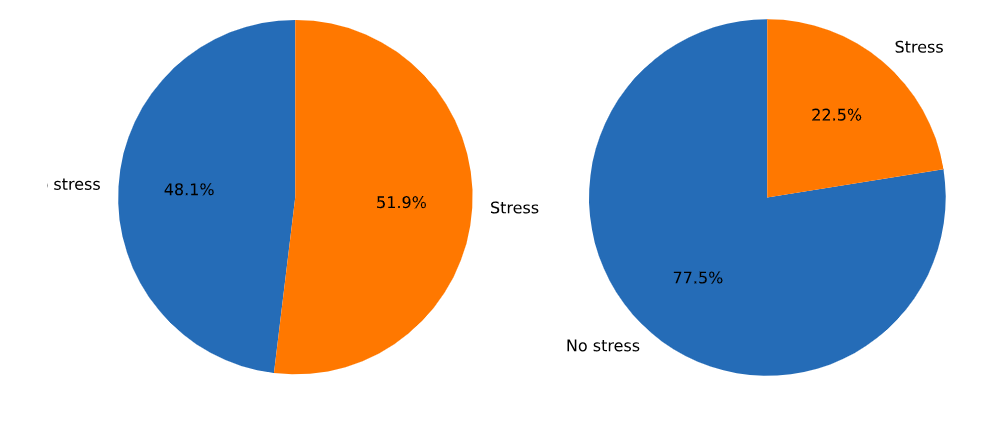
\includegraphics[width=7cm]{Graficos/stress.png}
    %\caption{Caption}
    \label{fig:enter-label}
\end{figure}



\begin{figure}[h]
    \centering
    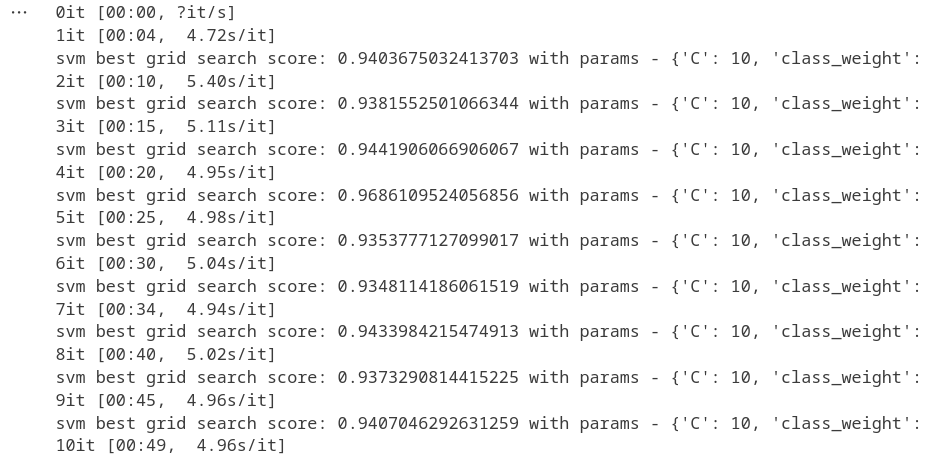
\includegraphics[width=7cm]{Graficos/capturaresutado.png}
    \caption{resultados}
    \label{fig:enter-label}
\end{figure}


\subsection{Métricas}

La mayoría de estos conjuntos de datos tienen un  números desigual de etiquetas de estrés/no estrés,por lo que usar la precisión como se uso en otros trabajos no es adecuado,para evitar sesgos  se elige una métrica de evaluación basada en el estudio  de   Sirko Straube et al. [ Sirko Straube et al, 2020], donde establece que la precisión equilibrada (BA)  es una opción adecuada para evaluar los resultados,ya que se quiere evaluar la capacidad de   distinguir las dos categorías para evaluar solamente  la precisión de detectar patrones de estrés.




%----- Figura dos columnas.
\begin{figure*}[!tb]
    \centering

    \caption{Ejemplo del \emph{aliasing} que se produce en una grilla con $N = 8$ nodos. Ambos modos
        ($k = 2$ y $k = 10$) toman los mismos valores en los puntos de la grilla.} \label{fig-2}
\end{figure*}
%----- Fin. Figura dos columnas.

\chapter{Conclusiones y trabajo futuro}
\hrule \bigskip \vspace*{1cm}
%------------------------------------------------------------------------


% \section{Conclusiones}

% Conclusiones que han podido ser cuantificadas o ampliamente
% deducibles (criterio lógico general) en base a TU TESIS.

% \section{Contribuciones}

% Con todo lo que has investigado, propuesto y/o desarrollado que haz
% conseguido obtener para cooperar con la solución del problema.

% \section{Trabajo futuro}

% Bueno ha estas alturas definitivamente te habrás dado cuenta que
% existe un montón de problemas que directa o indirectamente necesitan
% ser solucionados, es recomendable solo proponer y mostrar aquellos
% que en tu tesis haya una viabilidad cercana o muy relacionada, de
% tal forma pueda que una futura tesis(compañero) o estudios
% superiores le den continuidad.

Los modelos dependientes del usuario son mas preciso que los modelos independientes del usuario 
La conclusión está respaldada por las puntuaciones de BA del modelo  de detección de estrés entrenado



% \myappendix{Apendice}

\begin{singlespace}
\bibliographystyle{apalike}%plain
\mybibliography{biblio}
\end{singlespace}


\end{document}%%%%%%%%--------------------------------------------------------
